\chapter{导言}

学习计量经济学应该准备什么?怎么去做?首先推荐浙江大学
蒋岳祥老师的\href{https://www.bilibili.com/video/BV1es411W7KU?from=search&seid=3253765381861883959}{中高级计量经济学},厦门大学洪永淼老师的
\href{https://www.icourse163.org/course/XMU-1002606048}{高级计量经济学}  和
\href{https://www.bilibili.com/video/BV11t411A7bp}{概率论与统计学}。

\section{什么是计量经济学}

计量经济学是由挪威经济学家R.Fisher在三十年代首先创立的一门学科,是关于运用统计方法测量经济关系的艺术与科学,已经成为现代经济学的重要组成部分之一。

如果要给{\bf{计量经济学(Econometrics)}}下一个较为确切的定义,我们可以这样界定:

计量经济学是这样一门学科,它根据以往历史的经济资料与数据,从经济理论出发,运用数理统计的分析方法对经济关系建立经济计量模型,并依据所建立的模型对经济系统进行结构分析,经济预测和政策评价。所以计量经济学涉及数学学科中的统计学领域和经济学领域,统计学与经济理论是计量经济学的两块基石。

经济现象包罗万象,影响经济的因素有很多,如果我们企图将所有的因素作为研究的对象,我们可能什么结论也得不到,研究经济问题的一般方法是:我们总是选用最重要的因素变量而屏弃一些非本质的因素(变量),还需要了解哪些经济现象是有待解释的,哪些重要因素是有助于解释这些经济现象的,如何度量量化那些因素,并努力寻求它们之间存在的数量关系,并用统计推断来检验这些关系,
如\fref{fig:Econometrics}。

计量经济学的研究内容:随机现象,客观事物所反映的规律。

\begin{figure}[!htbp]
	\centering %居中
	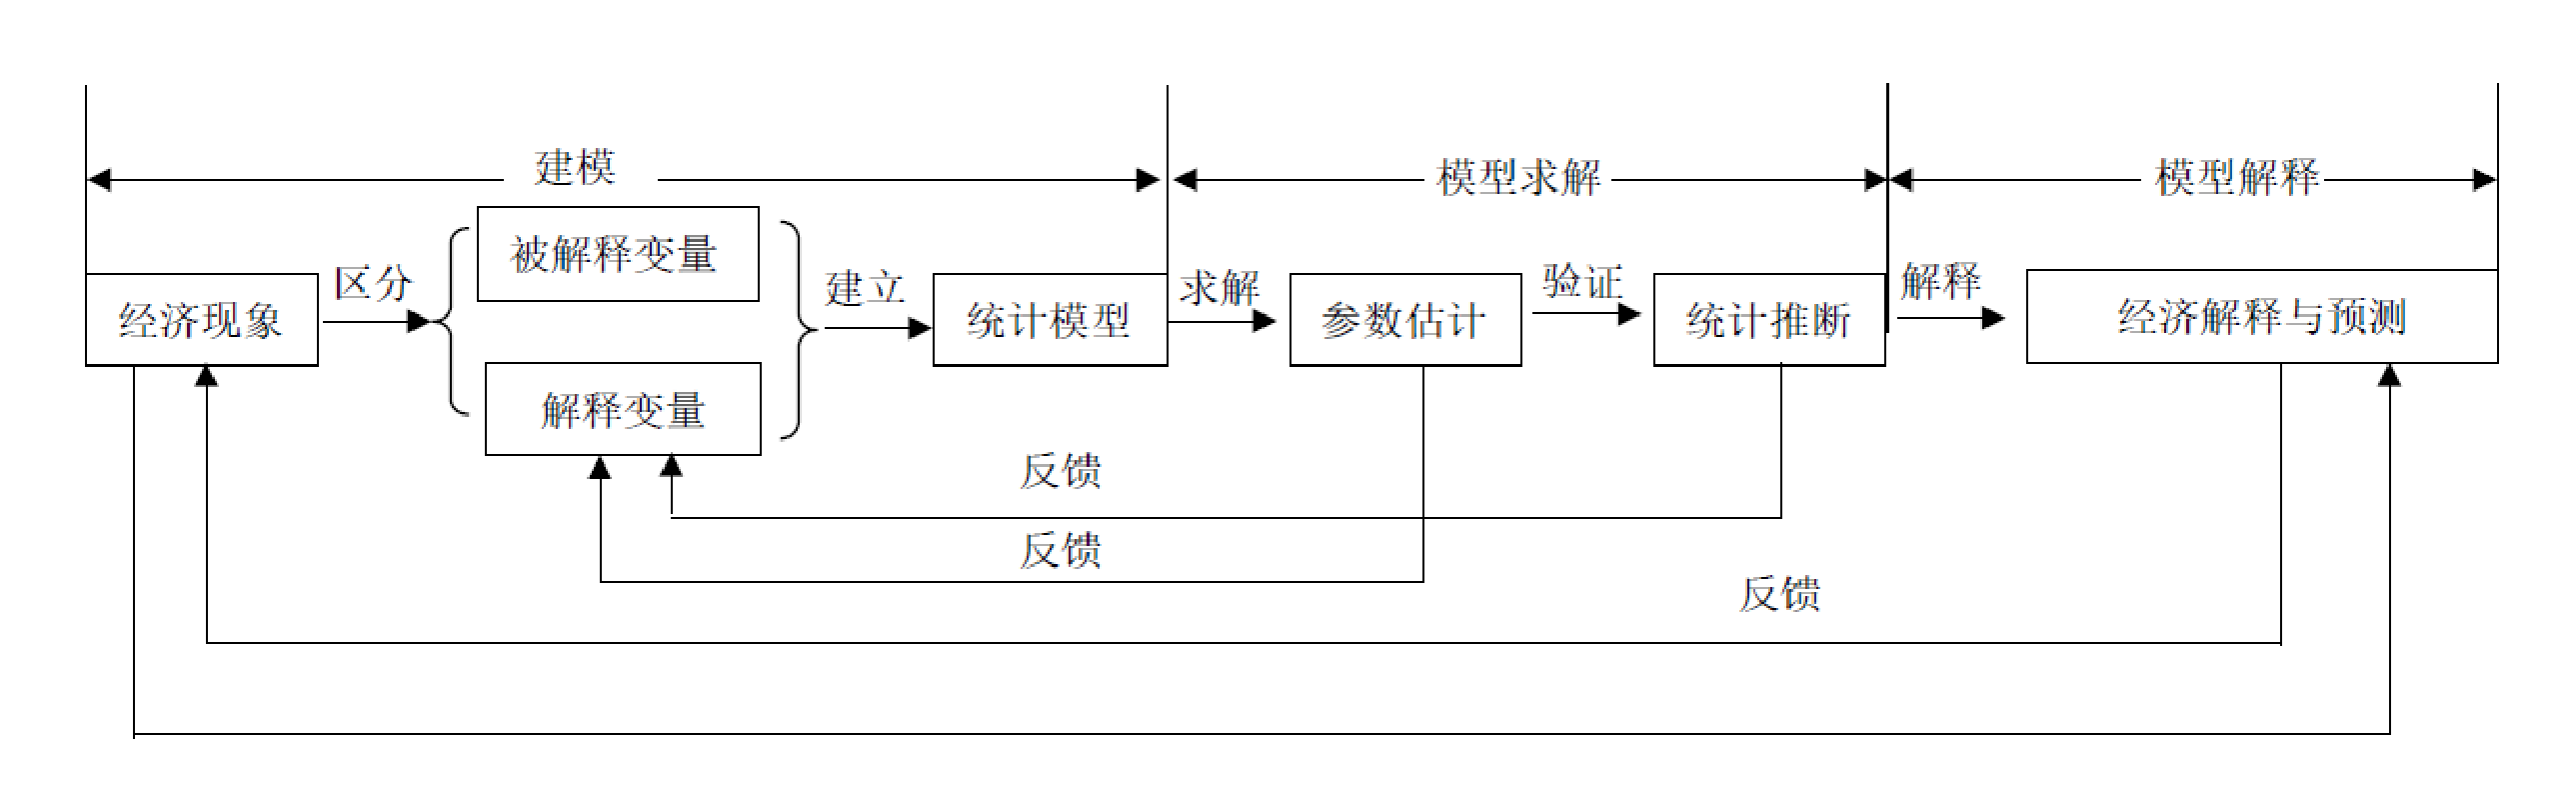
\includegraphics[width=0.9\textwidth]{Econometrics.eps}
	\caption{计量经济模型建立,求解,解释过程图}
	\label{fig:Econometrics}
\end{figure}

\section{随机现象的描述}
 工学和商学的思维模式与分析方法存在较大差异。一个是在确定下环境下少数可控变量关系的研究。另一个是研究在不确定性环境下无限且
不可控变量关系的问题。

实质上金融经济理论是研究不确定性的情况下,未来资源的如何最佳配置的问题。

银行为什么按揭贷款给年轻人?根据不同人来确定吗?未来的资产拿到今天来用。
研究随机现象是概率论与数理统计的知识。随机现象的处理,增加一个维度,例如基金经理投资成功的概率。
\begin{equation*}
	\lim_{n \to \infty} p^n =0  \qquad  \qquad  where \quad 0<p<1
\end{equation*}

研究对象的数据化,随机现象的描述——数据化。我们所看到的任何随机事件从理论上讲都可以通过将随机事件与数值联系。这样试验的结果就能有一个数来表示,
这个数是随着实验的结果的不同而变化,也即它是样本点一个函数,这种量被称为随机变量。

对于随机现象,最重要的是两件事,其一随机现象,其二出现结果的可能性。从而用来描述随机变量的大小变化和变化的可能性都可以量化。

随机现象 $A_1 , A_1 ,\cdots \cdots A_N $,为$ \boldsymbol{ A }$事件的集合体。$ I_{A_i} $ 表示事件是否发生。
	\begin{eqnarray}
		\boldsymbol{A} & =  & A_1  \cup  A_2 \cup A_3 \cup \cdots \cdots A_n  \notag\\ 
		& =  & \boldsymbol{A \Omega} = \boldsymbol{A}\sum_{i = 1}^{n} A_i = \sum_{i = 1}^{n} \boldsymbol{A} A_i \notag \\
		P(\boldsymbol{A}) & =  & P(\sum_{i = 1}^{n} \boldsymbol{A} A_i ) = 
		\sum_{i = 1}^{n} P(\boldsymbol{A} A_i) = \sum_{i = 1}^{n} P(\boldsymbol{A})P( A_i) \notag 
	\end{eqnarray}

\section{数据本质与统计规律}
概率论研究的分布函数,反映了事物变化和概率结合在一起。研究变量分为连续性变量,离散性变量。
计量经济学的三个定义,一是研究变量的分布函数,即古人所说的易,变化和概率(可能性)。
\begin{eqnarray}
	F(\mathrm {X} ) \quad & =  & P(\rm {X} \le \mathit{x} ) = \int_{-\infty }^{\mathit{x} } f(x)dx \notag \\
	F(\mathit{x_2}) - F(\mathit{x_1}) & =  &P(\mathit{x_1} <\rm X<\mathit{x_2}) \notag  \\
	\rm { Y }  & =  & X\beta + \varepsilon \qquad  \varepsilon \sim N(0,\sigma^ 2) 
\Longrightarrow Y ~\sim ~N(X\beta,\sigma^ 2)
\end{eqnarray}


计量模型估计$ \boldsymbol{\beta} , \ \ \varepsilon^2 \longrightarrow  $ 求Y的分布函数。
在均值附近变化一点,概率变化会很大。我国“古代思想”的概率论数据是基于随机现象的产生和发展得到的记录了事物发展的轨迹得到的数据,
不一定能够反映事物的本质不利用数据是否可以分析事物就是我们所说的玄学。

\subsection{数据的一般属性 } 

$  X_1,X_2,X_3,\cdots\cdots,X_n ~\sim ~F_{\theta} ~ (\mathit {x} ) $ 表明
$  X_1,X_2,X_3,\cdots\cdots,X_n  $ 独立同分布,

研究一个事物的要求分布函数,回归即是求分布函数,数据的分布($ \rm {X} \sim F_{\theta} (\mathit {x} $) )获得全样本是小概率事件,样本数据$ \Longrightarrow $ 母本数据。
\begin{eqnarray}
	\lim_{n \to \infty} \left \{ 
	\rm P \left (  X  =  \frac{1}{n} \sum X_i \le \mathit{x}  \right ) \right \}  
	 =  G_{\theta} \left( \mathit{x} \right) \sim \rm N(\mu,\sigma ^2) \notag 
\end{eqnarray}

$  n \to \infty $ 即为大样本,$ \rm \mu = \mathbb{E}(X) \sigma ^2 = var(X)$
平均属性$ \longrightarrow $ 平均的分布函数,查表时需进行标准化。哲学思想:天下乌鸦一般黑,事物随机现象的平均属性都服从正态分布。特例黑天鹅事件,
\begin{eqnarray}
	\rm P \left ( \frac{X-\mu}{\sigma }  \right )  \sim N (0,1) \notag
\end{eqnarray}

\subsection{数据的本质属性 } 

Fisher \&  Tippett 1928年已经完成,其极限分布只有三种类型。既所谓的极值分布是下列三种类型中的一种。最大值分布的特征事物的本质特征,事物最基本的本质。
\begin{eqnarray}
	\rm P \left [ max (X_1,X_2,X_3,\cdots \cdots X_n) \right ] < \it x \notag \\
	\lim_{n \to \infty} \rm P \left [ max (X_1,X_2,X_3,\cdots \cdots X_n) \right ] = ? \notag 
\end{eqnarray}
\begin{enumerate}
	\item \quad  Frechet分布 $ \Leftrightarrow   \rho > 0$
	\item \quad  Gumbel 分布 $ \Leftrightarrow   \rho < 0$
	\item \quad  Weibull分布 $ \Leftrightarrow   \rho = 0$
\end{enumerate}
\begin{equation*}
	 \rm min (X_1,X_2,X_3,\cdots \cdots X_n) = max (-X_1,-X_2,-X_3,\cdots \cdots -X_n)
\end{equation*} 

{\heiti{总结}}:假设研究对象是随机的,增加一个维度,用概率论的分布函数描述描述事物。

\begin{mydef}
研究对象的分布函数;
\end{mydef}
$$  \boldsymbol{\rm { Y }  = \beta^{\prime} X + \varepsilon } \qquad  \varepsilon \sim N(0,\sigma^ 2) 
      \Longrightarrow \boldsymbol{Y} \sim N(\boldsymbol{\beta^{\prime} X},\sigma^ 2) $$

\begin{mydef} 
	分部函数怎么确定?随机现象的平均属性基本相同,2008年金融危机后研究点,侧重于本质属性。MLE方法、OLS方法和矩估计等都可以估计参数 
	$ \boldsymbol{X} \sim F_{\theta} (\it \boldsymbol{x}) $
\[  \begin{cases}
		\rm P (\overline{X} < { \it x} )  \qquad \qquad \qquad  \ \ \qquad \Longrightarrow Law  \ \ of \ \ Large \ \ Numbers \\
		\rm P (max\left ( X_1,X_2\cdots \cdots X_n\right )  < { \it x} )   \Longrightarrow Law  \ \ of \ \ Large \ \ Numbers 
	\end{cases} \]

$ G_{X} (X) $ 可以用一个等式表示:
\[  H_{p}(\rm X) =  \begin{cases}
						\rm e^ {\left \{ -(1+\rho {\it x})^{-1/\rho} \right \} } \qquad   \qquad\Longrightarrow if  \ \ \rho \neq  0\\
						\rm e^ {\left \{ -e^{-x} \right \}}  \qquad \qquad  \qquad  \ \ \Longrightarrow if  \ \ \rho  =  0 
				    \end{cases} \]

$ \rho = 0 $ 状态就为太极(极限的极限),道的最高境界(无或双有)。数据是错的怎么办,利用古代人的做法,还原本质。
\begin{figure}[htb!]
	\centering
	\includegraphics[scale = 0.5 ]{Figs/Taiji.pdf}
	\caption{太极图}
\end{figure}

\end{mydef}

\section{数据的价值与《易经》}
回归包括线性回归和非线性回归,数据决定模型。计量经济学一般会求均值(一阶矩)和方差(二阶矩)。一般来说$ \overline{X}  \sim  N(\mu,\sigma^2) $。用样本去估计母体,t检验使用t统计量。为什么会使用t统计量。检验优先样本可以获得 $ \overline{x} \ \  , \ \   S^2 $

单个变量之间所表现出来的规律,但世界之间是有联系的,X对Y有无影响,$ \rm H_{0} : \boldsymbol{\beta} = 0 $ ,用t统计量。拒绝原假设时,$ \beta \neq 0 $。$ \beta = 0 $ 是不是小概率事件?
\begin{eqnarray}
	\boldsymbol{ Y  = \beta^{\prime} X + \varepsilon } \qquad  \varepsilon \sim N(0,\sigma^ 2) 
	\Longrightarrow \boldsymbol{Y} \sim N( \boldsymbol{\beta^{\prime} X},\sigma^ 2)   \notag \\ 
	\rm (X_1,Y_1) \quad  (X_2,Y_2) \quad  (X_3,Y_3)  \cdots \cdots (X_N,Y_N) 
	\Longrightarrow Regression \ \ Coefficient  \notag
\end{eqnarray}
	\begin{table}[htb!]
	\caption{两类错误}
	\centering
	\songti
	\begin{tabular}{c|c|c}
		\hline 检验状策 & $\mathrm{H}_{0}$ 为真 & $\mathrm{H}_{0}$ 非真 \\
		\hline 拒绝 $\mathrm{H}_{0}$ & 犯$ \rm\uppercase\expandafter{\romannumeral 1}$类错误 $(\mathrm{\alpha})$ & 正确 \\
		\hline 接受 $\mathrm{H}_{0}$ & 正确 & 犯 $ \rm\uppercase\expandafter{\romannumeral 2}$ 类错误 $(\beta)$ \\
		\hline
	\end{tabular}
    \end{table}

一个事情虽然说用很小,但未必不发生作用,发生时就会为黑天鹅事件,计量经济学的背景为不存在黑天鹅事件。
现实社会中一个政策把事物的性质可以发生改变。很多因素都存在着非回归的关系。

数据的两大属性:数据的一般属性和本质属性对应的反映事物的一般属性和本质属性,

任何真正反映事物发展轨迹的数据是和事物本质一样,有“性”,并同样存在同性恋的情况。
对于任何研究,首先要做定性分析,而非定量分析分析,任何事物都有“性”,“性”是事物的本质,而且可以做定量分析。
《易经》与统计学的关系,《易经》研究的是风险,规避统计学建立的模型分析和预测也是风险规避。
“易”是事物变化的统计规律,“易”是事物的变化和可能性。“易”变化的复杂和简单相统一,极限是科学的语言极限,是中心极限定理、小概率事件的基础。

\begin{myexample}
	传统文化为什么阻碍中国人的科学技术进步?中国偏向于小概率事件。
\end{myexample}
\begin{myexample}
	就业愿望的衡量。劳动参与率(Lobor Force Paticular Rate)。L为收益率,$ \varepsilon $ 为冲击。
	$$ LFPR = \alpha + \beta L + \varepsilon $$
\end{myexample}

可以有如下原假设: $ H_0 : \beta = 0 $ , $ H_0 : \beta < 0 $。将工资水平考虑到估计中,分析工资的挤出效应。
$$ LFPR = \alpha + \beta_1 L + \beta_2 FH + \varepsilon $$

{\heiti{计量经济学常用的表达式:}}
\begin{enumerate}[1)]
	\item $\varepsilon$ 假设
	\item $\hat{\alpha} \ \ \hat{\beta_1} \ \ \hat{\beta_2} $线性部分,$ \hat{\sigma^2} $随机部分
	\item $ H_0 : \beta_1 = 0 $ , $ H_0 : \beta_2 = 0 $
	\item $ H_0 : \beta_1 = \beta_2 =  0 $
	\item $ R^2 $ 拟合优度,判定系数
	\item 预测,随机现象。
\end{enumerate}

\subsection{回归的本质}

设随机变量$ \boldsymbol{\beta^{\prime} X, Y, X^{T}} =\left(X_{1}, \ldots, X_{m} \right) $是$ m $维随机向量,它是可以预先测量的,
希望通过$ \boldsymbol{X} $ 预测 $ \boldsymbol{Y} $, 也就是说要寻找一个函数$ \rm y= M \left(\it x_{1}, \ldots, \it x_{m}\right) $ 当X的观察值为x时,
就把$ \rm M(\it x) $作为对Y的预测值。当然一般总希望一个好的预测,其均方预测误差应达到最小。

均值处理随机性,$ \rm M(\it x) $与Y最大相关,此时相关系数最大。
\begin{eqnarray}
	\mathbb{E}[Y-L(X)]^{2} & = & \mathbb{E}[Y-M(X)]^{2} + \mathbb{E}[M(X)-L(X)]^{2}  \notag \\ 
	\rm \rho\left [ Y,M({\it x}) \right ] & = & \max_{L}\rho\left [ Y,L(X) \right ] \notag
\end{eqnarray}

设(X,Y)的分布密度函数是 $  f(x,y) $ , 设X的边际分布密度函数是 $  f_{1}(x) $ ,Y关于X的条件分布密度是:
\[ \rm Y = \begin{cases}
				f(x,y)/f_{1} (x)  \qquad \qquad f_{1} (x) \neq 0 \\
				0        \qquad  \quad  \qquad     \qquad \qquad f_{1} (x)= 0 
			\end{cases}  \]
%优化函数
	\begin{align*}
		& M(x) \underset{ \ \ = \ \ }{\Delta} E(Y / x)=\int y f(y / x) ~ d y\\
		&\mathbb{E}[Y-L(X)]^{2}=\iint \ldots \int[y-L(x)]^{2} f(x, y) ~ d x d y \\ 
		& 	= \iint \ldots \int[y-L(x)+M(x)-M(x)]^{2} f(x, y) ~ d x d y \\
		&	= \iint \ldots \int[y-M(x)]^{2} f(x, y) ~ d x d y\\
		&+2 \iint \ldots \int[y-M(x)][M(x)-L(x)] f(x, y) ~ d x d y\\
		&+\iint \ldots \int[M(x)-L(x)]^{2} f(x, y) ~ d x d y  \vspace{1em} \\
		\Longrightarrow \qquad
		& \iint \ldots \int[y-M(x)][M(x)-L(x)] f(x, y) ~ d x d y \\
		& =\iint \ldots \int[y-M(x)][M(x)-L(x)] f(y / x) f_{1}(x) ~ d y d x \\
		& =\int \ldots \int[M(x)-L(x)] f_{1}(x)\left[\int y f(y / x) ~  d y-M(x)\right] d x = 0
	\end{align*}
\begin{equation}
	\mathbb{E}[Y-L(X)]^{2} = \mathbb{E}[Y-M(X)]^{2} + \mathbb{E}[M(X)-L(X)]^{2}
\end{equation}

右边第一项与$ L(X) $无关,第二项大于等于零,它等于零的充要条件是$ M(X) = L(X) $, 
它表示当 $ M(X) = L(X) $时, $ \mathbb{E}[Y-L(X)]^{2} $达到最小值 $ \mathbb{E}[Y-M(X)]^{2} $。
在统计学上,我们称$ Y = M(X) = \mathbb{E}(Y|X)  $为Y关于X的回归曲线。
\begin{displaymath}
	min \ \  [Y - M(x)]^2 = \min_{L} \ \ [Y-L(x)]^2 
\end{displaymath}
% 定义定理写法
\begin{theorem}[条件均值]
	\begin{align*}
		M(x) & = \mathbb{E}(Y|X)	\\
		Y & = \mathbb{E}(Y|x) + [ Y-\mathbb{E}(Y|x) ] = \mathbb{E}(Y|x) + \varepsilon \ \ \ \ \mathbb{E}(\varepsilon) =  0 
	\end{align*}
\end{theorem}

 $ \mathbb{E}(\boldsymbol{\varepsilon}) \neq  0 $ 将会如何?当$ X,Y $满足二元正态分布时,可以得到一般线性回归,
 求 $ \boldsymbol{Y = \mathbb{E}(Y|x) + \varepsilon }$,即指导联合分布。
$$ \boldsymbol{Y} = F(\boldsymbol{\beta,X}) + \boldsymbol{\varepsilon} , \mathbb{E}(\boldsymbol{\varepsilon}) =  0,  
		\mathbb{E}(\boldsymbol{\varepsilon \varepsilon^{\prime}}) = \sigma^2 \boldsymbol{\Omega}  $$

  $ \mathbb{E} (\boldsymbol{\varepsilon \varepsilon^{\prime}} )$为协方差矩阵,
$ (\varepsilon_1,\varepsilon_2,\cdots,\varepsilon_n) $为样本点,OLS回归会假设服从正态性分布。随机变量之间的联系是通过协方差系数。
\begin{eqnarray}
	\rho_{XY}  & = & \frac{\mathbb{E}\Big((X-\mathbb{E}X)(Y-\mathbb{E}Y)\Big)}{\sqrt{DX}\sqrt{DY}} \notag \\
	\rm cov(\varepsilon_{i},X_{j} ) & = & 0 \notag \\ 
	\rm \rho_{Y,M({\it x})} ^2 & = &\frac{cov^2 \left [ \ \ {Y},E(Y|X) \ \  \right ] }{ var(Y)var\left [ \mathbb{E} (Y|X)\right ]} \notag \\ 
	& =  & \frac{cov^2 \left [ \ \ E(Y|X) ,E(Y|X) \ \  \right ] }{ var(Y)var\left [ E(Y|X)\right ]} \notag \\
	& =  & \frac{var\left [ E(Y|X)\right ] }{ var(Y)} = R^2 \notag \\
	\Longrightarrow \qquad \rm \widehat{R_{Y,\hat{Y}}^2} & =  &  \frac{SSR}{SST}  = \widehat{\rho_{Y,\hat{Y}}^2} 
\end{eqnarray}
 

统计学中求均值,方差,相关系数,$ \rho $为相关系数阵,是变量之间的关系网。
古典线性回归是对现实问题的简化再简化。样本数据一般会存在异方差问题,$ \sigma^2_1 \neq \sigma^2_2 $,如组间数据异方差。

自相关问题,一阶自回归模型。
\begin{displaymath}
	\boldsymbol{\Sigma} =\left(
	\begin{array}{ccccc}
	\sigma^{2} & \rho & \rho^{2} & \cdots & \rho^{n-1} \\ 
	\rho & \sigma^{2} & \rho & & \rho^{n-2} \\ 
	\rho^{2} & \rho & \sigma^{2} & & \vdots \\ 
	\vdots & & & \ddots & \rho \\ \rho^{n-1} & \cdots & & \rho & \sigma^{2}
	\end{array}  \right)
\end{displaymath}

ARCH(条件异方差),GARCH(广义条件异方差)。对 $ L(\alpha , \beta) $求偏导,得到
$ \widehat{\alpha}, \widehat{\beta} \Longrightarrow Y_{i} =  \widehat{\alpha} + \widehat{\beta} X_{i} + e_{i} $。
得到$ e_{1},e_{2},\ldots e_{n} $ 检验 $ \varepsilon  \sim  N(0,\sigma^2) $
$$  \boldsymbol{\Sigma} = \left(\begin{array}{cccc}
 \sigma_{1}^{2} & 0 & \cdots & 0 \\ 
 0 & \sigma_{2}^{2} & & \vdots \\ 
 \vdots & & \ddots & 0 \\ 0 & \cdots & 0 & \sigma_{n}^{2}
 \end{array} \right) $$
\begin{displaymath}
	Y_{i} = \alpha + \beta X_{i} + \varepsilon_{i}  \qquad
	L(\alpha , \beta) = \sum_{i=1}^n(Y_{i} -\alpha -\beta X_{i} )^2
\end{displaymath}
\begin{enumerate}
	\item$  X_{1},X_{2},\ldots  $\ \ $ \Longrightarrow Y $,利用联合分布$ f(X_{1},X_{2},\ldots X_{m})  \Longrightarrow L(\cdot) $
	\item $ Y = \beta X + \varepsilon \qquad H_0 : \beta_1 =0 / H_0 : \beta_2 =  0 $
	\item $ \varepsilon_1,\varepsilon_2,\ldots \varepsilon_n $,
			对于PRF,$ \mathbb{E}( \boldsymbol{\varepsilon} ) = 0  $
			$ \mathbb{E}( \boldsymbol{\varepsilon \varepsilon{\prime}} )  $= $ \sigma^2 \boldsymbol{\Omega} $是否满足。
	\item OLS。 $ L(\alpha , \beta) = \sum_{i=1}^n(Y_{i} -\alpha -\beta X_{i} )^2 \Longrightarrow Y 
	     =  \widehat{\alpha} + \widehat{\beta} X + e (Sample  \ \  Regression \ \ Function) $理解为条件回归+波动,一般有几个假定,就会有几个检验。
\end{enumerate}


\section{计量经济学实例}
\subsection{消费}

学过经济学中凯恩斯经济理论的人都知道,理论上说消费和收入存在着密切的联系,如果C表示消费,Y表示收入。则C与Y的关系,可用消费函数表示:
\begin{equation}
	C = f(Y)
\end{equation}

这样的函数满足:

1) \quad 边际消费倾向(MPC)位于0和1之间; 

2) \quad 平均消费倾向(APC)是随着收入的增加而减少。

\begin{eqnarray}
\frac{d \dfrac{C}{Y}}{d Y} & = & \frac{d\left(C \cdot \frac{1}{Y}\right)}{d Y} \notag \\ 
& = & \frac{d C}{d Y} \cdot \frac{1}{Y}-\frac{1}{Y^{2}} C \notag \\ 
& = & \frac{1}{Y}\left( \frac{d C}{d Y} -\frac{C}{Y}\right) \notag =\frac{1}{Y}\left( MPC -APC\right)<0
\end{eqnarray}

在现实经济社会中,消费与收入之间的关系很难确切地用方程(1)表示收入,我们所能采集到的数据往往受到这样那样的影响,我们可用随机扰动 来表示这些影响,所以,我们要对方程(1)要作适当调整,于是消费和收入之间的关系可以写成如下形式:
\begin{equation}
	C = f(Y,\varepsilon)
	\label{eq 1.5.2}
\end{equation}

其中$\varepsilon$是随机扰动。满足凯恩斯条件的 $\varepsilon$很多,无法枚举穷尽,但我们可以大致将它们分为线性模型与非线性模型两类。

\textbf{1. \quad 线性模型(Linear Model)}

方程\eqref{eq 1.5.2}的一个最简单的情况,是C与Y的线性关系,即:
\begin{equation}
	C = \alpha + \beta Y + \varepsilon
\end{equation}

如果我们现在从历史记录中或观察到N个样本,即($Y_t , C_t $ ),$ t=1,2,\cdots \cdots N $,于是我们有如下一组方程:
\begin{align*}
	&\mathrm{C}_{1}=\alpha+\beta \mathrm{Y}_{1}+\varepsilon_{1}\\
	&\mathrm{C}_{2}=\alpha+\beta \mathrm{Y}_{2}+\varepsilon_{2}\\
	&\cdots\cdots \\
	&\mathrm{C}_{\mathrm{N}}=\alpha+\beta \mathrm{Y}_{\mathrm{N}}+\varepsilon_{\mathrm{N}} 
\end{align*}

\textbf{2. \quad 非线性模型(Nonlinear Model)}

一般情况下,方程\eqref{eq 1.5.2}都是非线性的情况。现在我们假设0< $ \nu $ <1, MPC>0 ,即该模型满足凯恩斯的两个条件,这就是一个典型非线性模型。例如:
\begin{equation*}
	\mathrm{C}=\alpha+\beta \mathrm{Y}^{\nu}+\varepsilon
\end{equation*}
\subsection{奥肯定律}

奥肯定律:失业率每上升1\%,实际GDP下降2\%,这是线性回归的结果。

\subsection{Solow模型}
 带有$\mu$的Solow模型,西方经济理论在中国未必行得通,因为具体分布不同。希克斯提出中性技术条件。超越对数的生产函数,  \quad $\alpha$ 劳动的产出弹性,$\beta$资本的产出弹性。
	\begin{eqnarray}
		Y & = & A(t)f(L,K) =A_{0}e^{\mu t}f(L,K)  \nonumber \\
		\ln Y & = & lnA_{0} + \mu t + \ln f(L,K) 
	\end{eqnarray}
	\begin{eqnarray}
		\frac{d\ln Y} {dt} & = & \mu + \frac{d\ln f(L,K)}{dt}  \nonumber   \\
		\frac{d\ln Y} {Ydt}& = & \mu + \frac{\partial f}{f\partial L} \frac{dL}{dt} +\frac{\partial f}{f\partial K} \frac{dK}{dt} \nonumber \\ 
		& = & \mu +\frac{L}{f} \frac{\partial f}{\partial L} \frac{1}{L} \frac{dL}{dt} +
		\frac{L}{f} \frac{\partial f}{\partial K}\frac{1}{K} \frac{dK}{dt} \nonumber 
	\end{eqnarray}
	\begin{eqnarray}
		\frac{d \ln Y} {Ydt} & = & \mu + \frac{L}{A_{0}e^{\mu t}f} \frac{A_{0}e^{\mu t} \partial f}{\partial L} 
		\frac{1}{L} \frac{dL}{dt} +\frac{L}{A_{0}e^{\mu t}f} \frac{A_{0}e^{\mu t} \partial f}{\partial K}\frac{1}{K} \frac{dK}{dt} 
	\end{eqnarray}
	\begin{eqnarray}	
	\frac{\Delta Y} {Y}	& \stackrel{dt = 1}{=} &  \mu + \alpha \frac{\Delta L} {L} + \beta \frac{\Delta K} {K} \nonumber   \\
		1 &	=  &  \frac{\mu} {\Delta Y/Y} + \alpha \frac{\Delta L/L} {\Delta Y/Y} + \beta \frac{\Delta K/K} {\Delta Y/Y} \nonumber  
	\end{eqnarray} 
$$ \frac{\mu} {\Delta Y/Y}  \ \ is \ \ the \ \ Technological \ \ innovation $$ 

CD函数,$\alpha+ \beta = 1$ ,现对规模效应做检验,则$\beta = 1 - \alpha$
$$ 	\frac{\Delta Y} {Y}	=  \mu + \alpha \frac{\Delta L} {L} + (1 - \alpha) \frac{\Delta K} {K} \nonumber $$